\tikzstyle{majorStyle}=[shape = circle, minimum size = 6pt, inner sep = 2.2pt, draw]
\tikzstyle{major}=[shape = circle, minimum size = 6pt, inner sep = 2.2pt, draw]
\tikzstyle{minorStyle}=[shape = rectangle, minimum size = 6pt, inner sep = 2.2pt, draw]
\tikzstyle{minor}=[shape = rectangle, minimum size = 6pt, inner sep = 2.2pt, draw]
\tikzstyle{labeledStyle}=[shape = rectangle, minimum size = 6pt, inner sep = 2.2pt, draw]
\tikzstyle{VertexStyle} = []
\tikzstyle{EdgeStyle} = []
%\tikzstyle{unlabeledStyle}=[shape = circle, minimum size = 6pt, inner sep = 1.2pt, draw, fill]
\begin{figure}[htb]
\begin{center}
\subfloat[]{\makebox[.33\textwidth]{
\begin{tikzpicture}[scale = 6]
\Vertex[style = major, x = 0.45, y = 0.95, L = \small {$4$}]{v0}
\Vertex[style = major, x = 0.15, y = 0.75, L = \small {$3$}]{v1}
\Vertex[style = major, x = 0.35, y = 0.75, L = \small {$3$}]{v2}
\Vertex[style = major, x = 0.55, y = 0.75, L = \small {$4$}]{v3}
\Vertex[style = major, x = 0.55, y = 0.55, L = \small {$3$}]{v4}
\Edge[label= \small {$e$}, , labelstyle={auto=right, fill=none}](v0)(v1)
\Edge[](v2)(v0)
\Edge[](v2)(v3)
\Edge[](v3)(v0)
\Edge[](v4)(v3)
\draw[white] (0,.475)--(0,0.49);
\end{tikzpicture}
}}
%\subfloat[Figure 2]{\makebox[.5\textwidth]{
%\begin{tikzpicture}[scale = 8]
%\Vertex[style = major, x = 0.400, y = 0.900, L = \small {$u$}]{v0}
%\Vertex[style = minor, x = 0.150, y = 0.700, L = \small {$v_1$}]{v1}
%\Vertex[style = minor, x = 0.300, y = 0.700, L = \small {$v_2$}]{v2}
%\Vertex[style = major, x = 0.500, y = 0.700, L = \small {$v_3$}]{v3}
%\Vertex[style = major, x = 0.650, y = 0.700, L = \small {$v_4$}]{v4}
%\Vertex[style = minor, x = 0.650, y = 0.550, L = \small {$w$}]{v5}
%\Edge[](v1)(v0)
%\Edge[](v2)(v0)
%\Edge[](v2)(v3)
%\Edge[](v3)(v0)
%\Edge[](v4)(v0)
%\Edge[](v5)(v4)
%\end{tikzpicture}
%}}
\subfloat[]{\makebox[.33\textwidth]{
\begin{tikzpicture}[scale = 7]
%\begin{scope}[xshift=.7cm,yshift=.1cm]
\Vertex[style = major, x = 0.5, y = 0.849, L = \small {$4$}]{v0}
\Vertex[style = major, x = 0.200, y = 0.650, L = \small {$3$}]{v1}
\Vertex[style = major, x = 0.400, y = 0.650, L = \small {$3$}]{v2}
\Vertex[style = major, x = 0.600, y = 0.650, L = \small {$4$}]{v3}
\Vertex[style = major, x = 0.800, y = 0.650, L = \small {$4$}]{v4}
\Vertex[style = major, x = 0.550, y = 0.449, L = \small {$3$}]{v6}
\Vertex[style = major, x = 0.649, y = 0.449, L = \small {$3$}]{v5}
\Vertex[style = major, x = 0.800, y = 0.449, L = \small {$3$}]{v7}
\Edge[label= \small {$e$}, , labelstyle={auto=right, fill=none}](v0)(v1)
\Edge[](v2)(v0)
\Edge[](v3)(v0)
\Edge[](v4)(v0)
\Edge[](v5)(v3)
\Edge[](v6)(v3)
\Edge[](v7)(v4)
\end{tikzpicture}
}}
%\end{scope}
%}}
%
%\subfloat[]{\makebox[.5\textwidth]{
%\begin{tikzpicture}[scale = 8]
%\Vertex[style = major, x = 0.500, y = 0.849, L = \small {$u$}]{v0}
%\Vertex[style = minor, x = 0.400, y = 0.650, L = \small {$v_1$}]{v2}
%\Vertex[style = minor, x = 0.500, y = 0.650, L = \small {$v_2$}]{v1}
%\Vertex[style = major, x = 0.600, y = 0.650, L = \small {$v_3$}]{v3}
%\Vertex[style = major, x = 0.800, y = 0.650, L = \small {$v_4$}]{v4}
%\Vertex[style = minor, x = 0.500, y = 0.449, L = \small {$w_1$}]{v6}
%\Vertex[style = minor, x = 0.699, y = 0.449, L = \small {$w_2$}]{v5}
%\Edge[label= \small {$e$}, , labelstyle={auto=right, fill=none}](v0)(v2)
%\Edge[](v1)(v0)
%\Edge[](v3)(v0)
%\Edge[](v4)(v0)
%\Edge[](v4)(v5)
%\Edge[](v5)(v3)
%\Edge[](v6)(v3)
%\end{tikzpicture}
%}}
\subfloat[]{\makebox[.33\textwidth]{
\begin{tikzpicture}[rotate=90,scale=7]
%\begin{tikzpicture}[yshift=.253cm,xshift=2.8cm,rotate=90,scale=7]
\Vertex[style = major, x = 0.35, y = 0.80, L = \small {$3$}]{v0}
\Vertex[style = major, x = 0.65, y = 0.80, L = \small {$3$}]{v1}
\Vertex[style = major, x = 0.50, y = 0.65, L = \small {$4$}]{v2}
\Vertex[style = major, x = 0.50, y = 0.95, L = \small {$4$}]{v3}
\Vertex[style = major, x = 0.50, y = 0.50, L = \small {$4$}]{v4}
\Vertex[style = major, x = 0.50, y = 0.35, L = \small {$3$}]{v5}
\Edge[](v2)(v0)
\Edge[label= \small {$e$}, , labelstyle={auto=right, fill=none}](v2)(v1)
\Edge[](v3)(v0)
\Edge[](v3)(v1)
\Edge[](v4)(v2)
\Edge[](v5)(v4)
\draw[white] (.26,.55)--(.27,.55);
\end{tikzpicture}
}}
%\end{scope}
\end{center}
\caption{Each configuration is reducible by deleting edge $e$.
(The number at each vertex specifies its degree in G.)\label{fig:hiltonzhao}}
\end{figure}
%Vertices drawn as circles have degree 4 in $G$ and vertices drawn as rectangles
%have degree 3 in $G$.  
